\section{Definitions}

WebAssembly, shortened to Wasm, is a binary instruction format for a stack-based virtual machine ~\cite{wasm-core-spec}. It is a platform-agnostic binary format, meaning that it will run the same exact instructions across whatever machine it operates on. ~\cite{wasm-polkadot-wiki}

`asm.js` was Wasm precursor, but browser vendors like Mozilla, Google, Microsoft, and Apple focused on the Wasm design. The main goal was to create a binary format with some mandatory features: compact, support for streaming compilation and sanboxed execution.

Wasm is currently a compilation target for a lot of high level language. This allows many different languages to enter the web-world, in both client and server sides, but also in completely different applications.

Examples are plugins. Imagine an application able to execute custom script developed by the user: if those scripts are in Wasm then the High-Level language used to develop those plugins is not constrained to a single one but to all the languages that are able to compile to Wasm.

Wasm main design goals, as specified in the Wasm specification introduction ~\cite{wasm-core-spec}, are:
\begin{description}[font=$\bullet$ \scshape\bfseries]
  \item[Fast] Its design allows to create executors with so less overhead that the execution is almost as fast as native code
  \item[Safe] It is completely memory-safe as long as the executor is  behaving correctly, sandboxing the execution properly
  \item[Well-defined] The definition of the binary format makes it easy to create a valid executor that makes the code behave correctly
  \item[Hardware-independent] The compilation process is independent from the architecture that will run the code
  \item[Platform-independent] It can be compiled and executed on all modern architectures, embedded systems or applications (like browsers)
  \item[Open] There is a simple way to interoperate the with executor/environment
\end{description}

Other important considerations are made on the efficiency and portability. The specification describes Wasm also as: compact, modular, efficient, streamable, and parallelizable.

% Something not clear at first look is \"modular\", it means that the program can be split into smaller parts and those can be transmitted, cahed and consumed separately.

In the following chapters the words `executor` or `embedder` have the same meaning.

\section{Specifications}

The specification does not make any assumption on the embedder. This makes it completely unconstrainted as far as it implements all the defined instruction set, binary encoding, validation, and execution semantics ~\cite{wasm-core-spec}.

Wasm is stack-based. This means that the instruction set is very different from the standard architecture's bytecode that are normally registered-based. Wasm has also a one-to-one text representation other than the normal binary representation, which makes the code less compact but almost human readable.

All the concepts present in the specifications are very high-level even if it is a low level language. The most relevant are:

\begin{description}[font=$\bullet$ \scshape\bfseries]
  \item[Values]
        Wasm has only four data types: integers and floating points (following IEEE 754 standard) both 32 and 64 bits
  \item[Instructions]
        Being a stack based language every instruction works implicitly on a stack but there is a general division between:
        \begin{itemize}
          \item Simple Instructions, performing basic operations on data
          \item Control Flows, allowing to follow some high-level language control flow having nested blocks
        \end{itemize}
  \item[Traps]
        Those are instructions which immediately aborts the execution. The termination is not handled by wams itself but by the embedder
  \item[Functions]
        Being so new, this assembly-like language allows users to work with functions abstracting some of the assembly's complexity
  \item[Linear Memory]
        This is where the communication between the code and the environment happens: the linear memory is a contiguous area of memory given to the code. This memory is very crucial for the security considerations that we will see later.
  \item[Modules]
        A Module is the logical container of the code. Every Wasm code is made by a single module.
  \item[Exports] Once the module is instantiated all the defined exports are callable from the embedder, examples of possible exports are functions or global variables.
  \item[Imports] Wasm can import things from the embedder. The more common examples are the functions provided from the outside that are callable from the Wasm code
  \item[Embedder]
        Wasm needs the embedder to be executed. Itsthe main jobs are:
        \begin{itemize}
          \item loading and initiate a new module
          \item provide imports
          \item manage exports
        \end{itemize}
\end{description}

Other important concepts explained in the specification are Wasm phases:

\begin{description}[font=$\bullet$ \scshape\bfseries]
  \item[Decoding]
        Decode the binary format to the specified abstract syntax. The implementation could also compile directly to machine code.
  \item[Validation]
        A decoded module has to be valid. The validation consists in check a set of well-formed conditions to guarantee that the module is meaningful and safe ~\cite{wasm-polkadot-wiki}
  \item[Execution]
        Execution is made by two sub-phases:
        \begin{itemize}
          \item Instantiation, set up state and execution stack of a module
          \item Invocation, calling a function provided by the module to start the effective execution
        \end{itemize}
\end{description}

\section{Execution}

Wasm specifications try to be unbreakable but at the end everything depends on the embedder's implementation: if it is not secure then Wasm execution itself is not.

\subsection{Execution Types}

There are two main categories of execution types: compilation and interpretation, those are then made by multiple sub-categories based on the technical details. The main difference is: in compilation the Wasm code is re-compiled to the architecture's bytecode and then natively executed on the machine. The interpretation, instead, uses a Virtual Machine to parse the Wasm code and execute it inside of the machine.

\

Every type has its own advantages but also requires different tricks to make everything secure. One important thing provided by Wasm is an articulated test suite to check the correctness of the embedder.~\cite{wasm-testsuite}

The common divisor for every compilation type of execution is the transpilation of a stack-based bytecode to a register one; something similar happens also in the interpretation because the Wasm code is stack-based but generally it needs to be executed on a register-based one.

In Wasm there are multiple stacks:
\begin{itemize}
  \item the Value Stack, used implicitly by Wasm to store temporary data or passing values to functions
  \item  the Shadow Stack, this is not directly related to Wasm but used by many toolchains in the compilation to Wasm.
\end{itemize}

Passing values around only by values is not always efficient and in Wasm you don't have access directly to the value stack being only implicitly used by all the common instructions. The compiler uses the Shadow Stack, allocated in the Linear Memory (explained later), to put information in it and pass around pointer to this stack as value in the Value Stack.

\begin{figure}[h]
  \centering
  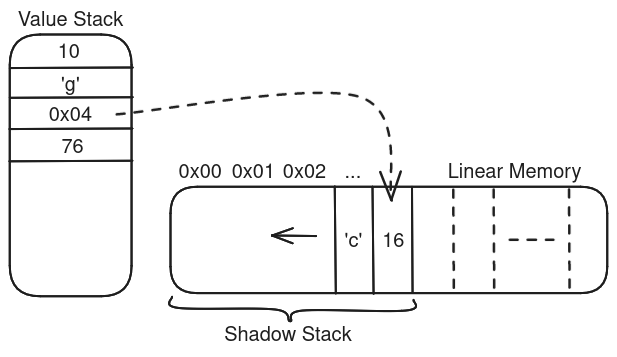
\includegraphics[width=0.5\linewidth]{value_and_shadow_stack.png}
  \caption{Value and Shadow Stack}
  \label{fig:value-shadow-stack}
\end{figure}

Those two stacks are present in the Wasm code but when it needs to be translated to the final bytecode the compiler tries to elide every access to the Value Stack allocating everything needed in the registers. Registers are limited though, so is impossible to use only them and the native stack of the embedder will be used if needed.

\

The main types of execution used in blockchains are: Ahead Of Time Complication (AOT), Just In Time Compilation (JIT), Single Pass Compilation and generally Interpretation


\begin{description}[font=$\bullet$ \scshape\bfseries]
  \item[AOT]
        is the standard compilation, all the code is compiled and then executed.
  \item[JIT]
        is a dynamic compilation type where the bytecode is compiled only when needed. The compiler needs to create first an intermediate representation, to be later able to compile the different parts only if the execution requires to. A really simple example to make is: we have a program with two entry point, function A and B. The JIT process will cover the understanding of the structure, recognize the two functions and compile only the needed one, either A or B.

        Lots of optimizations are already been done in the first phase of compilation, from the High-Level language to Wasm. In the second phase (runtime compilation) the main goal is to compile only the required parts to the machine-specific bytecode not caring too much about adding optimizations.
  \item[SPC]
        is a restriction of AOT Compilation, the complexity of the compilation must be O(n) so the Wasm bytecode will be scanned through only once. Like every other compilation methods here the objective is not to create efficient final code but to create the final bytecode as fast as possible.
  \item[Interpretation] % ???
        is the easiest way to execute Wasm, which becomes like any other interpreted language executed by a specialized Virtual Machine.

\end{description}

\subsection{Embedders}

There are multiple embedders able to execute Wasm using techniques not even explained before. We will focus on three specific embedders commonly used in blockchains: Wasmtime, Wasmi and Wasmer.

Those three cover all the techniques just explained:

\begin{description}[font=$\bullet$ \scshape\bfseries]
  \item[Wasmtime]
        is a stand alone Wasm environment but it could be also used as library to create a Wasm environment in your bigger application. Wasmtime offers multiple features, it accepts Wasm in text or binary format and you're able to used JIT or AOT types of execution.
  \item[Wasmi]
        ~\cite{wasmi} is an efficient Wasm interpreter with low-overhead and support for embedded environment such as Wasm itself.

        There are multiple ways to interpret code. Wasmi makes a first Wasm bytecode pass to produce another stack-based bytecode, called WASMI IR (Intermediate Representation). Thereafter this representation is interpreted by a Virtual Machine, even with this transpilation it is only 5 times slower then the compilation to the native bytecode of the architecture.

        \item[Wasmer] has a lot of features, both AOT and JIT but in particular it implements a single pass compiler for all the most important architectures.
\end{description}

\section{Security guarantee}

Wasm principle aim is to be extremely secure. The specifications describes a lot of ways to achieve that feature, but the security guarantee depends mostly on the execution. WebAssembly is designed to be translated into machine code running directly on the host’s hardware, so it can be sent to someone and executed freely, (e.g., in browsers). We are running Wasm our machines every day, so security is a main concern.

Executing Wasm is potentially vulnerable to side channel attacks on the hardware level ~/cite{wasm-core-spec} and isolation is the only way to secure the execution.  The embedder translates one-by-one every instructions to native instructions on your computer, but nothing is dangerous if the code has no access to the environment where is executed.

The problem is that a completely isolation makes Wasm useless, so there must be a way to communicate with the environment or  have access to it, but those features are extremely limited and designed to be secure.

\subsection{Linear Memory}

From WebAssemply you have direct access to raw bytes, but where are  those bytes allocated? Wasm uses a MemoryObject provided by the embedder to describe the only accessible memory, besides the stack: the linear memory.~\cite{linear-memory}

Wasm does not have pointer types. Values in the linear memory are accessed as a vector, where the first index of the memory is 0.

Wasm, for security reasons that will be explained in the next chapters, works in a 32-bit address space. This makes usable only 4GiB of memory. Being the position of Linear Memory unknown to the Wasm blob every load or store to the memory is made passing through the embedder that will also do bounds checks to make sure the address is inside the Wasm Linear Memory.

\begin{figure}[h]
  \centering
  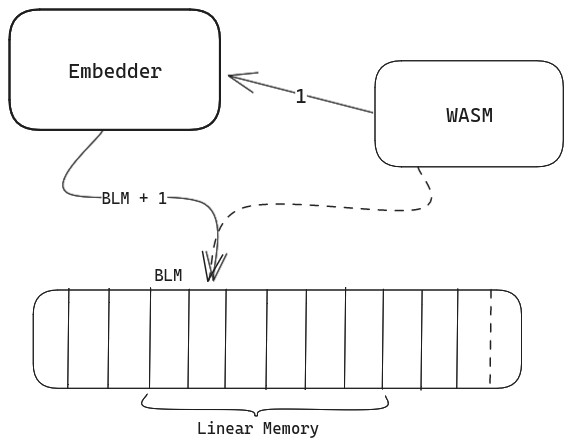
\includegraphics[width=0.5\linewidth]{linear_memory.png}
  \caption{BLM: Base Linear Memory Pointer}
  \label{fig:linear_memory}
\end{figure}

This level of control makes it impossible to have memory leaks in the environment during the Wasm execution because there is a complete memory isolation. ~\cite{linear-memory}

\subsection{Communication in a sandboxed environment}

We just described how Wasm provides no ambient access to the computing environment in which the code is executed ~\cite{wasm-core-spec}, thanks to a mix of Wasm design choice and embedder implementation. But how  then does the interaction with the environment work?

Every interaction can be done by a set of functions provided by the embedder and imported in the Wasm module~\cite{wasm-core-spec}. Those functions are called Host Functions and allow the Wasm code to access to resources, operating system calls or any other types of computation offered by the embedder. Generally the Exports provided by Wasm that are usable and callable from the embedder are called Runtime API.

\begin{figure}[h]
  \centering
  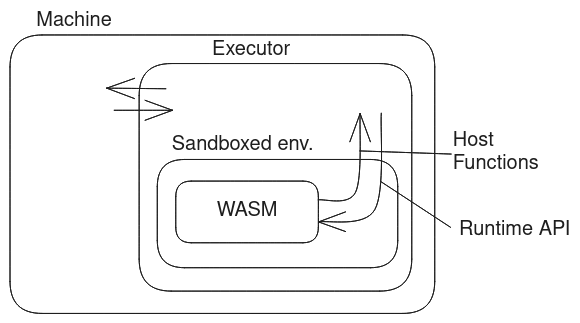
\includegraphics[width=0.5\linewidth]{env_communication.png}
  \caption{Environment communication}
  \label{fig:env-communication}
\end{figure}

\subsection{Wasmtime Security guarantee}

Wasmtime is widely used in different environments and as we will see in the next chapter one of those is the polkadot ecosystem.

Wasmtime main goals is to execute untrusted code in a safe manner.~\cite{wasmtime-book}

Some features that makes executing Wasm by Wasmtime secure are just inherited by the Wasm specifications. Some examples are: the callstack is inaccessible, pointers are compiled to offsets into linear memory, there's no undefined behavior and every interaction with the outside world is done through imported and exported functions.~\cite{wasmtime-book}

Wasmtime adds  a lot of mitigations to those features to limit risks:
\begin{itemize}
  \item Linear memories are preceded with a 2GB guard region  by default
  \item Wasmtime will zero the memory used by a WebAssembly instance after it's finished.
  \item Wasmtime uses explicit checks to determine if a WebAssembly function should be considered to stack overflow
  \item The implementation language of Wasmtime, Rust, helps catch mistakes when writing Wasmtime itself at compile time
\end{itemize}
